\documentclass[aspectratio=169]{beamer}
\usetheme{Boadilla}

%\usetheme{Warsaw}
%\setbeamercovered{transparent}
\beamertemplatetransparentcoveredhigh
\usepackage[portuges]{babel}
\usepackage[latin1]{inputenc}
\usepackage{lmodern}
\usepackage[T1]{fontenc}
\usepackage{hyperref} 
\usepackage{wrapfig}
\usepackage[portuguese, linesnumbered, vlined, titlenumbered, ruled]{algorithm2e}

\newcommand{\eng}[1]{\textsl{#1}}
\newcommand{\cod}[1]{\texttt{#1}}

\title[Apresenta��o]{Curso Intelig�ncia Artificial: do Zero ao Infinito}
\author[Frederico Oliveira]{Object Detection Data Augmentation}
\institute[UFMT]{Universidade Federal de Mato Grosso}
\date{}
%\titlegraphic{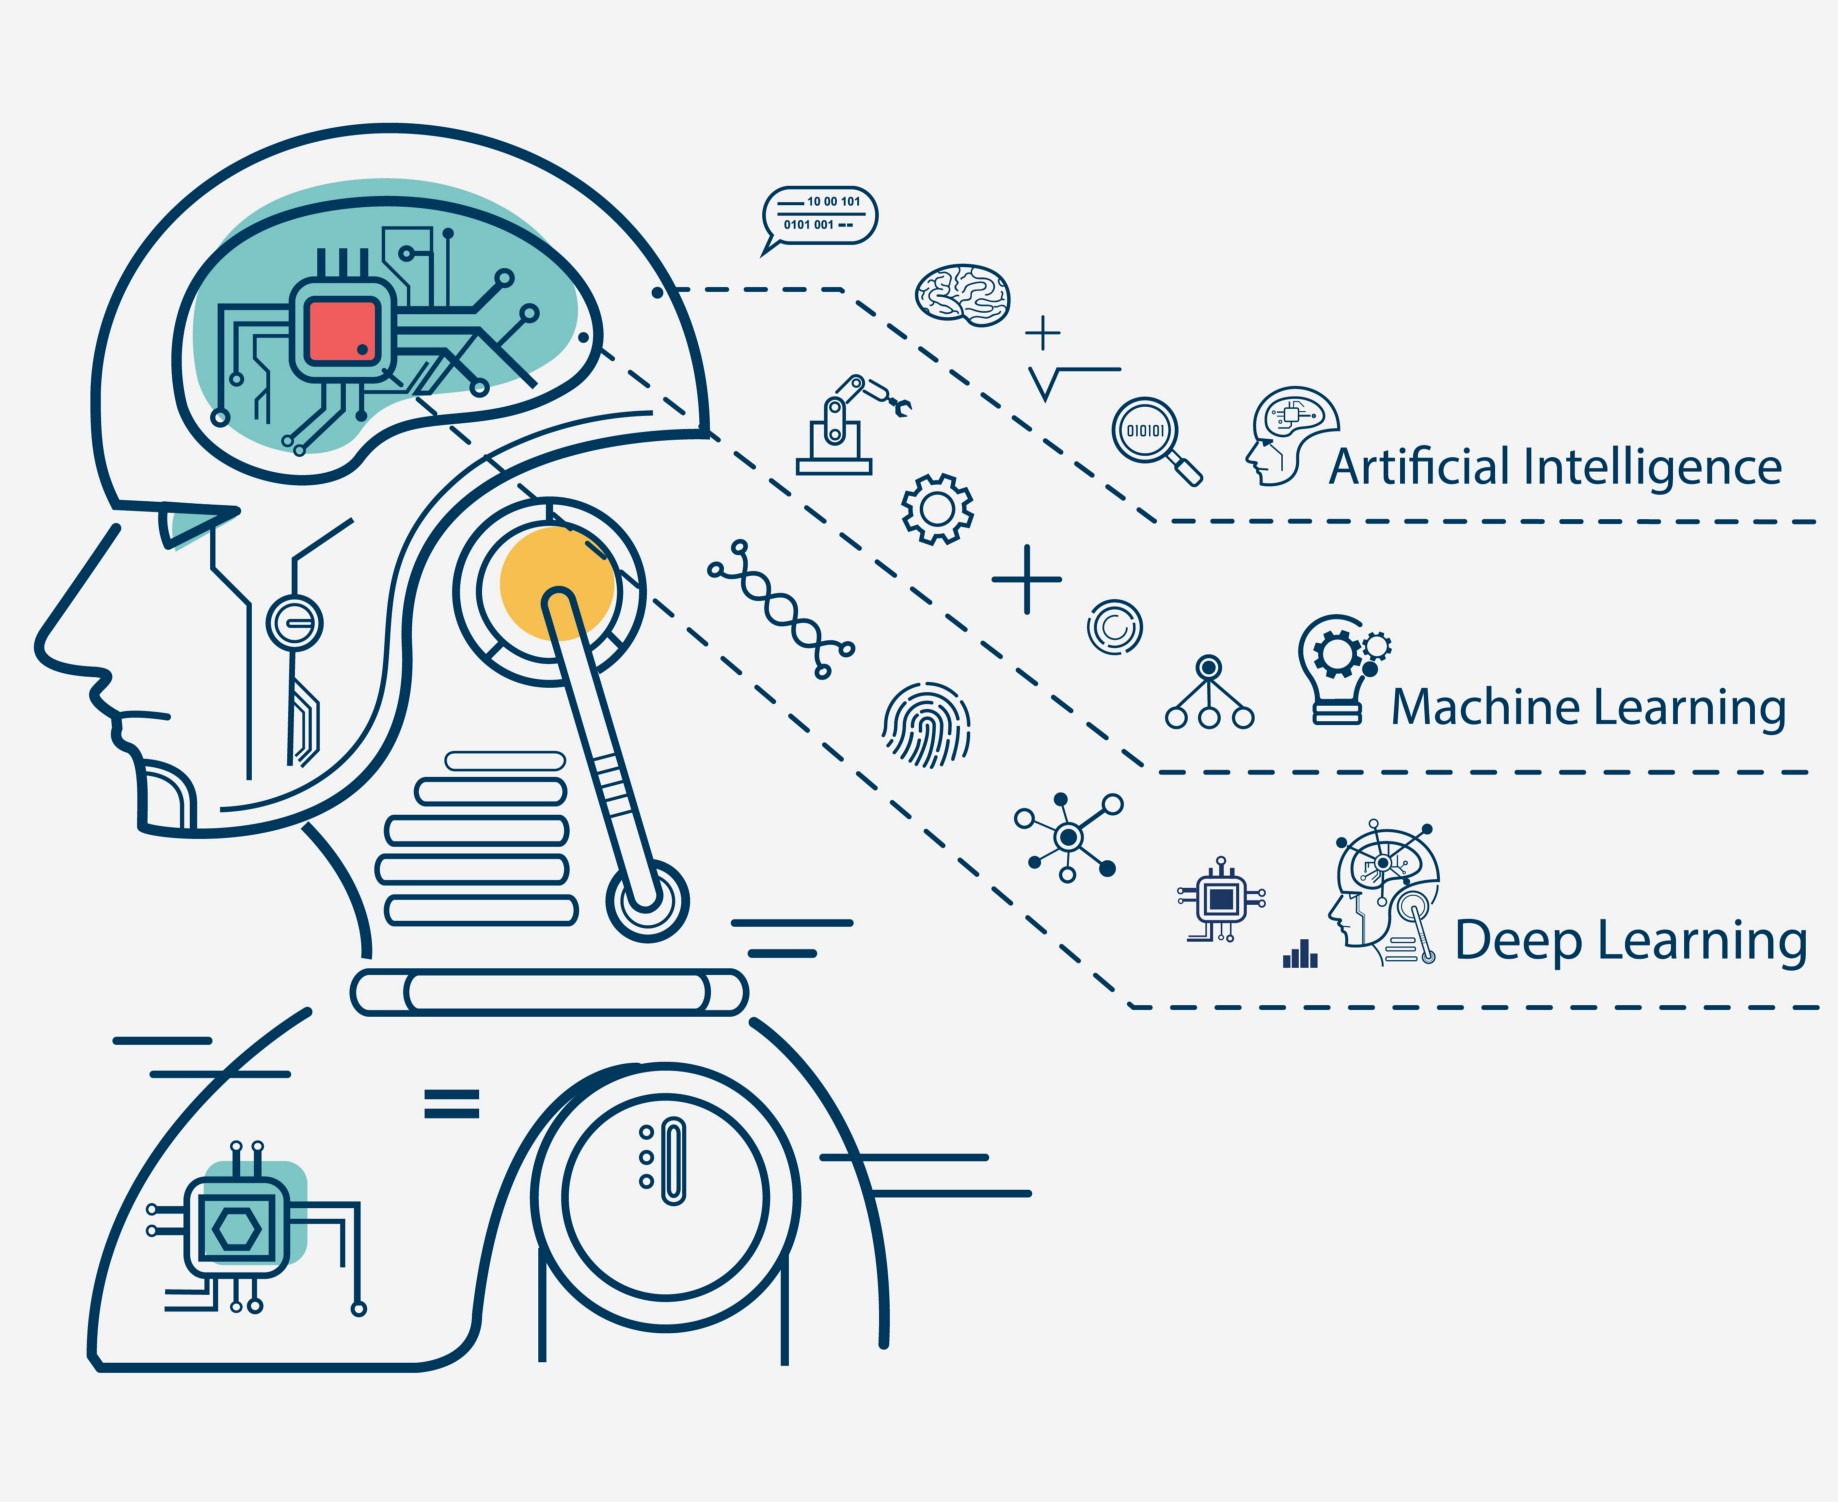
\includegraphics[width=\textwidth,height=.5\textheight]{imgs/intro.jpeg}}
%\usebackgroundtemplate{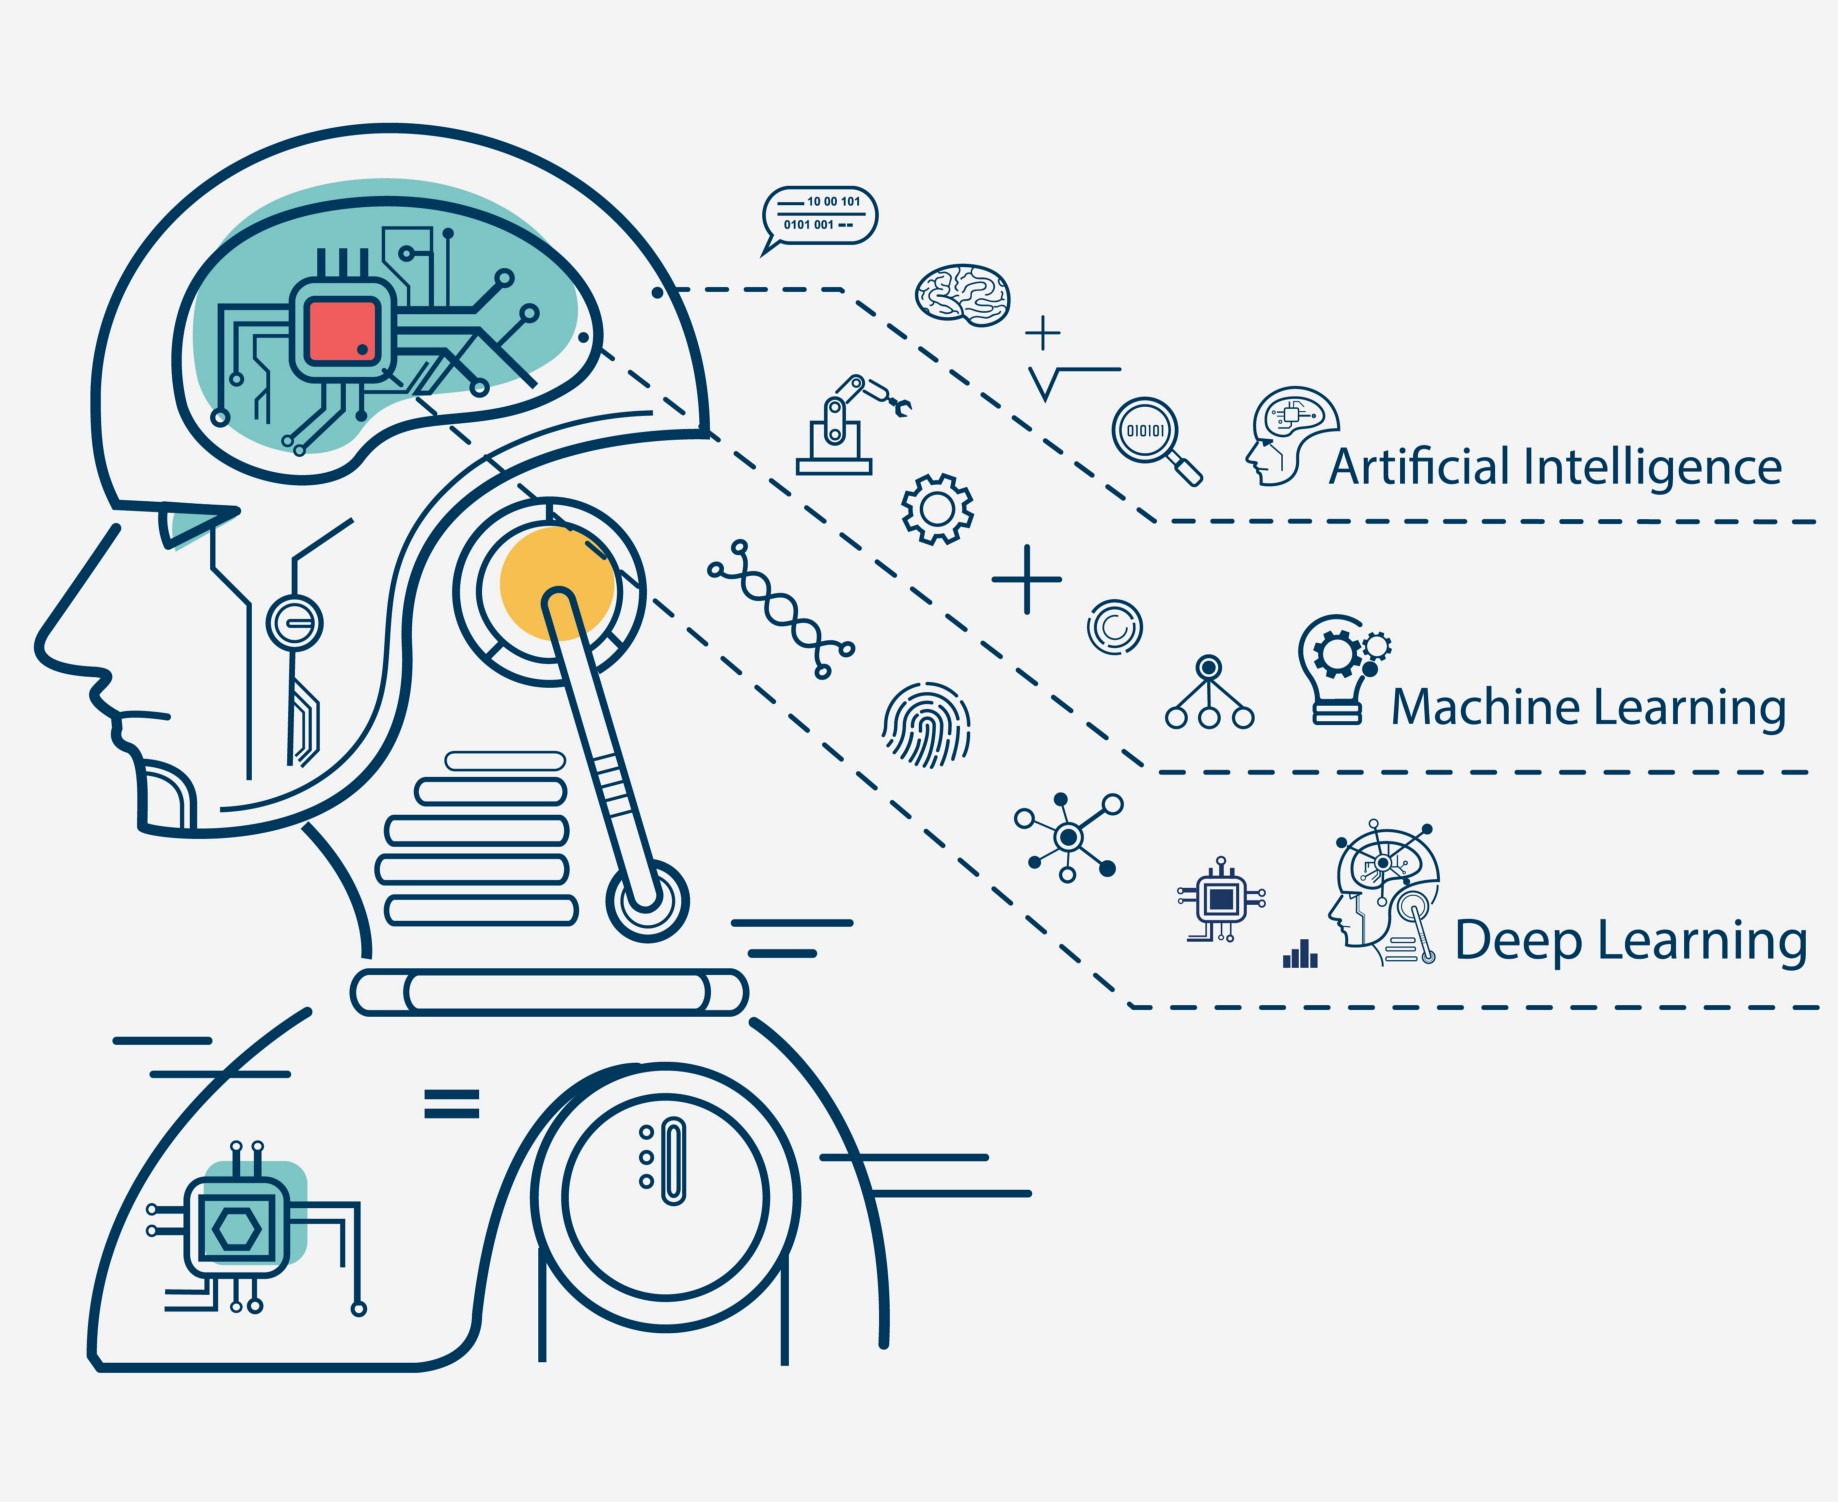
\includegraphics[width=\paperwidth]{imgs/intro.jpeg}}
\begin{document}

\begin{frame}[plain]
  \titlepage
\end{frame}

%%%%%%%%%%%%%%%%%%%%%%%%%%%%%%%%%%%%%%%%%%%%%%%%%%%%%%%%%%%%%%%%%%%%%%%%%%%%%%%%%%%%%%%%%%%%%%%%%%%%%%%%%%%%%%%%
%\section*{Roteiro}
%%%%%%%%%%%%%%%%%%%%%%%%%%%%%%%%%%%%%%%%%%%%%%%%%%%%%%%%%%%%%%%%%%%%%%%%%%%%%%%%%%%%%%%%%%%%%%%%%%%%%%%%%%%%%%%%

\begin{frame}
  \frametitle{Agenda}
  \tableofcontents
\end{frame}

%%%%%%%%%%%%%%%%%%%%%%%%%%%%%%%%%%%%%%%%%%%%%%%%%%%%%%%%%%%%%%%%%%%%%%%%%%%%%%%%%%%%%%%%%%%%%%%%%%%%%%%%%%%%%%%%
\section{Introdu��o}
%%%%%%%%%%%%%%%%%%%%%%%%%%%%%%%%%%%%%%%%%%%%%%%%%%%%%%%%%%%%%%%%%%%%%%%%%%%%%%%%%%%%%%%%%%%%%%%%%%%%%%%%%%%%%%%%

\begin{frame}{Object Detection Data Augmentation}{O que � data augmentation?}
\begin{figure}[h]
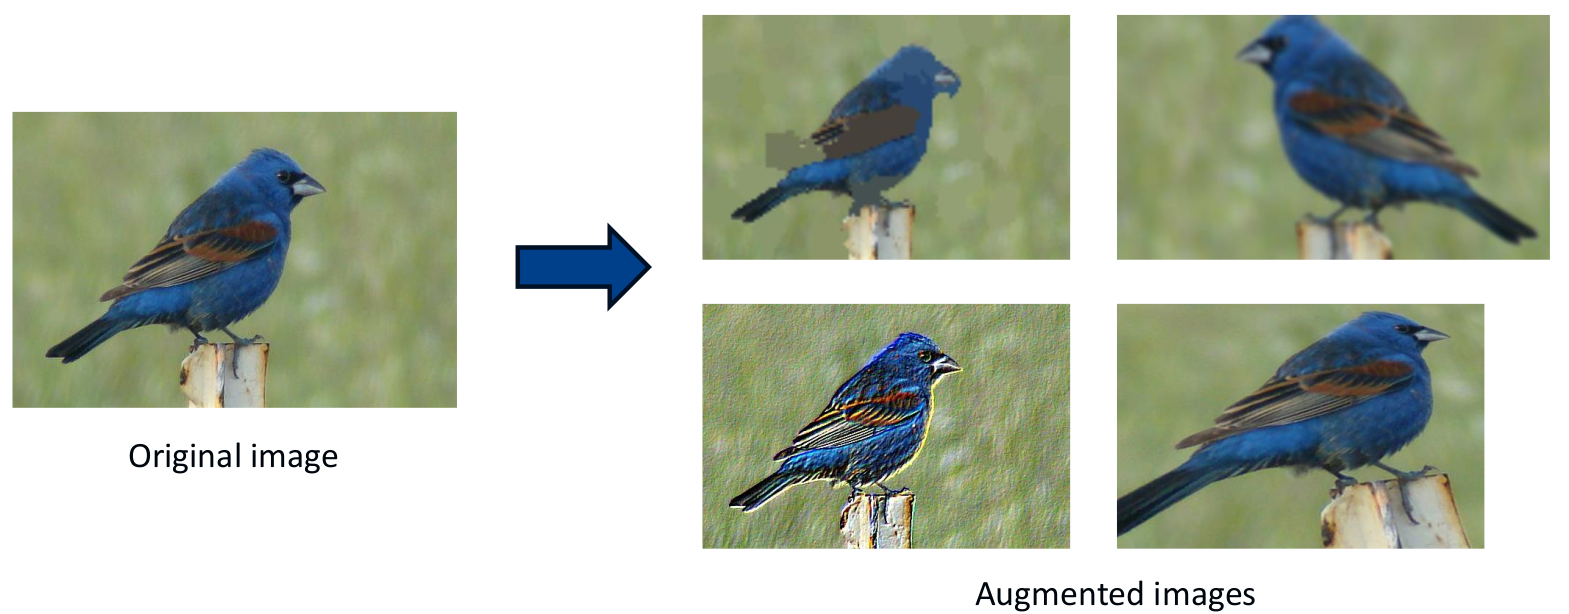
\includegraphics[width=8cm]{imgs/augmented_images.png}
\end{figure}

Cria um novo conjunto de dados modificando as imagens existentes
\end{frame}

%%%%%%%%%%%%%%%%%%%%%%%%%%%%%%%%%%%%%%%%%%%%%%%%%%%%%%%%%%%%%%%%%%%%%%%%%%%%%%%%%%%%%%%%%%%%%%%%%%%%%%%%%%%%%%%%

\begin{frame}{Object Detection Data Augmentation}{Por que usar data augmentation?}
\begin{itemize}
\item Aumenta o tamanho do dataset
\begin{itemize}
\item Previne overfitting
\item Aumenta a robustez das {\it features} extra�das
\item Aumenta a variedade dos ambientes visuais
\end{itemize}
\item Resolve o desbalanceamento entre as classes
\begin{itemize}
\item Desbalancemaneto de classes causa um enviesamento do modelo � classe dominante
\end{itemize}
\end{itemize}

\end{frame}

%%%%%%%%%%%%%%%%%%%%%%%%%%%%%%%%%%%%%%%%%%%%%%%%%%%%%%%%%%%%%%%%%%%%%%%%%%%%%%%%%%%%%%%%%%%%%%%%%%%%%%%%%%%%%%%%

\begin{frame}{Object Detection Data Augmentation}

\begin{figure}[h]
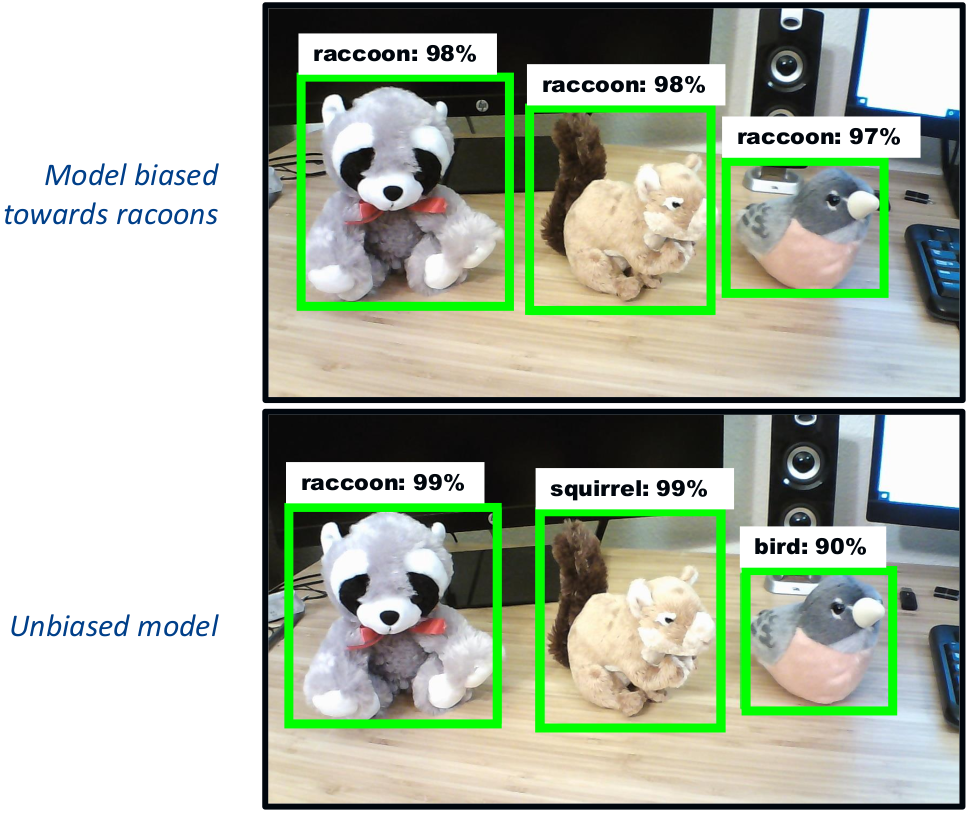
\includegraphics[width=8cm]{imgs/biased_model.png}
\end{figure}

\end{frame}

%%%%%%%%%%%%%%%%%%%%%%%%%%%%%%%%%%%%%%%%%%%%%%%%%%%%%%%%%%%%%%%%%%%%%%%%%%%%%%%%%%%%%%%%%%%%%%%%%%%%%%%%%%%%%%%%
\section{M�todos}
%%%%%%%%%%%%%%%%%%%%%%%%%%%%%%%%%%%%%%%%%%%%%%%%%%%%%%%%%%%%%%%%%%%%%%%%%%%%%%%%%%%%%%%%%%%%%%%%%%%%%%%%%%%%%%%%

\begin{frame}{Object Detection Data Augmentation}{M�todos para Data Augmentation}
\begin{figure}[h]
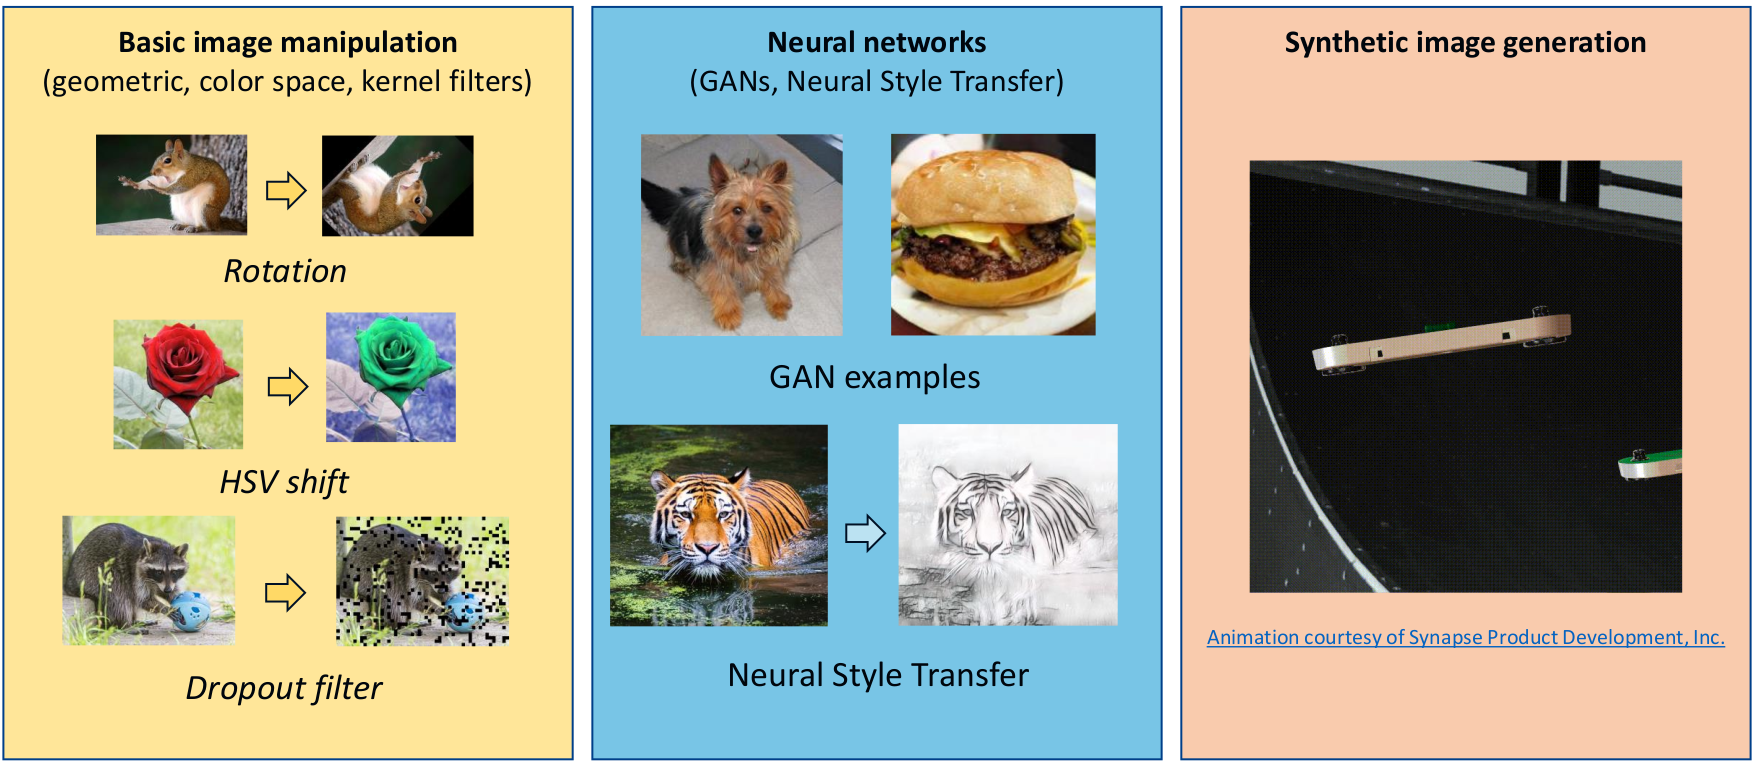
\includegraphics[width=14cm]{imgs/methods_for_data_augmentation.png}
\end{figure}

\end{frame}

%%%%%%%%%%%%%%%%%%%%%%%%%%%%%%%%%%%%%%%%%%%%%%%%%%%%%%%%%%%%%%%%%%%%%%%%%%%%%%%%%%%%%%%%%%%%%%%%%%%%%%%%%%%%%%%%

\begin{frame}{Object Detection Data Augmentation}{Synthetic Data Augmentation}
\begin{figure}[h]
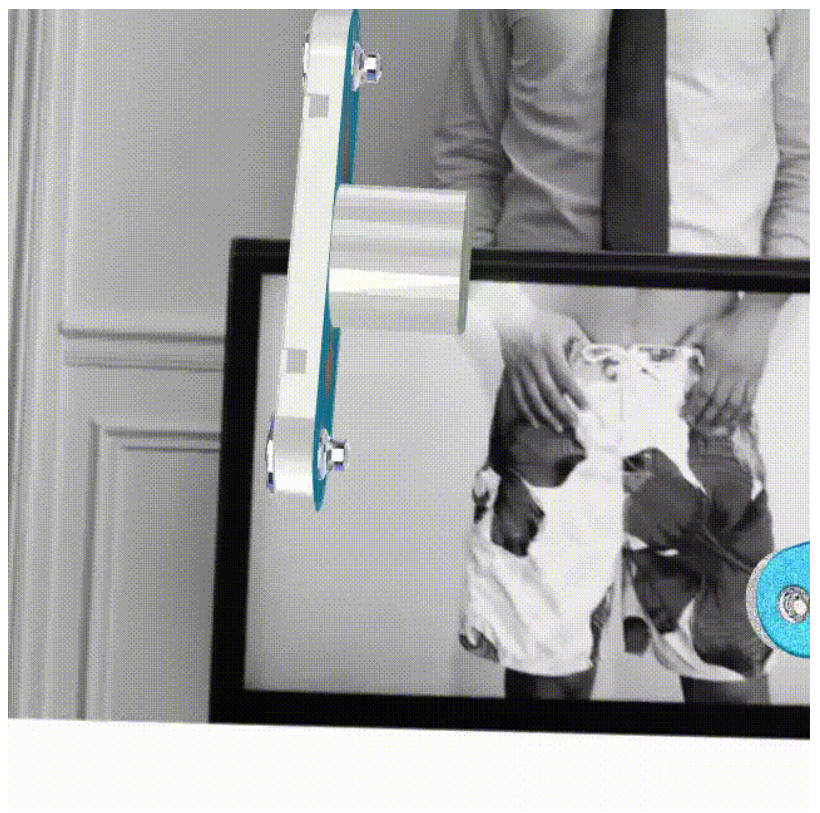
\includegraphics[width=3cm]{imgs/syn_data_aug1.png}
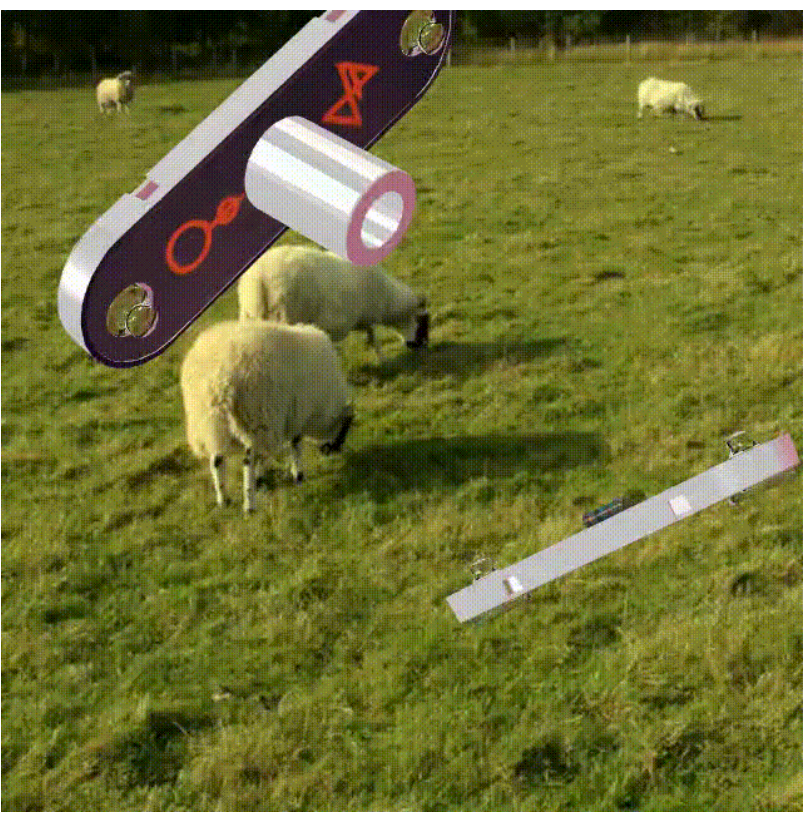
\includegraphics[width=3cm]{imgs/syn_data_aug2.png}
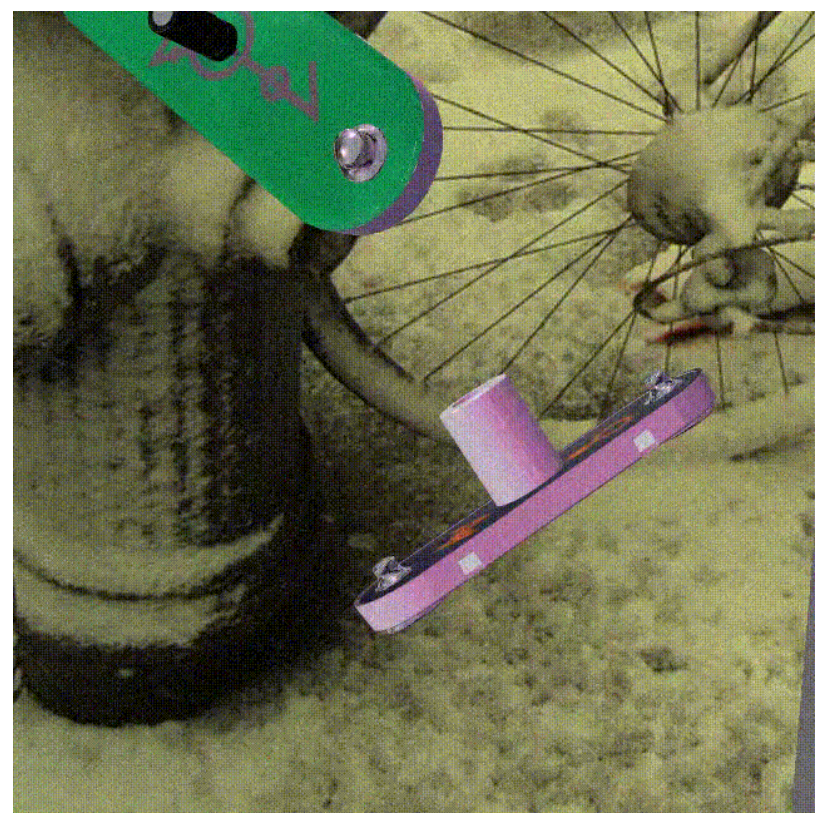
\includegraphics[width=3cm]{imgs/syn_data_aug3.png}
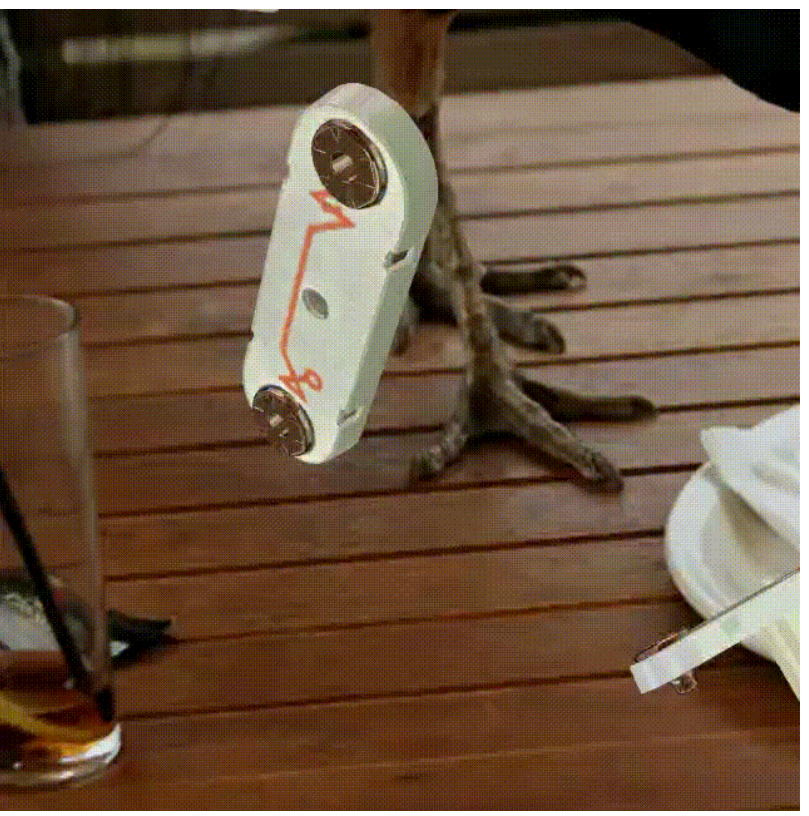
\includegraphics[width=3cm]{imgs/syn_data_aug4.png}
\end{figure}

\vspace{1cm}
\tiny{Fonte: \url{https://blog.synapse.com/post/automation-ar-and-jobs-a-demonstration}.}
\end{frame}

%%%%%%%%%%%%%%%%%%%%%%%%%%%%%%%%%%%%%%%%%%%%%%%%%%%%%%%%%%%%%%%%%%%%%%%%%%%%%%%%%%%%%%%%%%%%%%%%%%%%%%%%%%%%%%%%

\begin{frame}{Object Detection Data Augmentation}{Desafios}
{\it Data Augmentation} para {\bf Object Detection} � mais desafiador que {\bf Image Classification}:
\begin{itemize}
\item N�o transforma apenas a imagem, mas tamb�m as coordenadas do {\it bounding box}.
\item Precisa garantir que a transformac�o n�o destruir� o {\it bounding box}.
\end{itemize}
\end{frame}

%%%%%%%%%%%%%%%%%%%%%%%%%%%%%%%%%%%%%%%%%%%%%%%%%%%%%%%%%%%%%%%%%%%%%%%%%%%%%%%%%%%%%%%%%%%%%%%%%%%%%%%%%%%%%%%%

\begin{frame}{Object Detection Data Augmentation}{Desafios}
\begin{figure}[h]
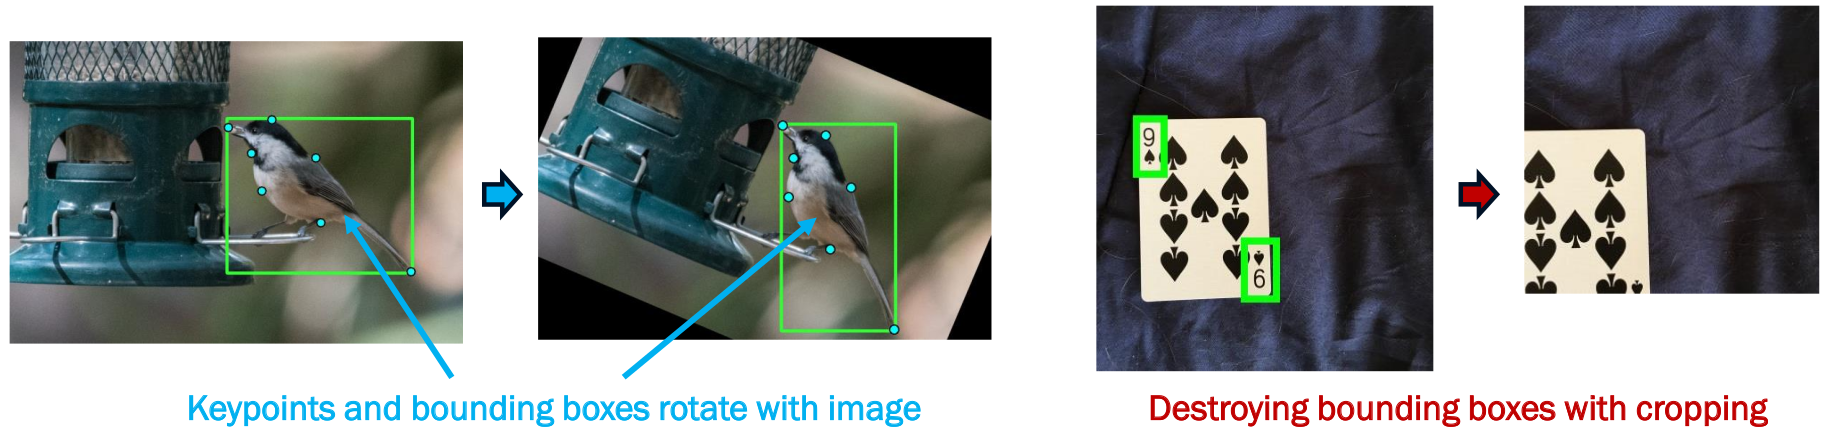
\includegraphics[width=14cm]{imgs/bounding_boxes_challenges.png}
\end{figure}
\end{frame}

%%%%%%%%%%%%%%%%%%%%%%%%%%%%%%%%%%%%%%%%%%%%%%%%%%%%%%%%%%%%%%%%%%%%%%%%%%%%%%%%%%%%%%%%%%%%%%%%%%%%%%%%%%%%%%%%

\begin{frame}{Object Detection Data Augmentation}{Ferramentas}
\begin{itemize}
\item[{
\includegraphics[width=7mm]{imgs/github.png}}] Open-source GitHub libraries: \href{https://github.com/aleju/imgaug}{Imgaug}, \href{https://github.com/mdbloice/Augmentor}{Augmentator}, \href{https://albumentations.ai/}{Albumentations}
\begin{itemize}
\item Pros: Free, well-documented, good examples
\item Cons: May become unavailable or stop being maintained
\end{itemize}
\item[{
\includegraphics[width=7mm]{imgs/opencv.png}}] OpenCV has image manipulation functions for manually creating augmentations
\begin{itemize}
\item Pros: Free, tight and flexible control over augmentation parameters
\item Cons: Have to write everything yourself
\end{itemize}
\item[{
\includegraphics[width=7mm]{imgs/tf.png}}] TensorFlow Object Detection API provides augmentation options to automatically use during preprocessing
\begin{itemize}
\item Pros: Free, easy to use (zero-effort)
\item Cons: Not many operations available, may stack poorly with existing augmentations in dataset
\end{itemize}
\end{itemize}

\end{frame}

%%%%%%%%%%%%%%%%%%%%%%%%%%%%%%%%%%%%%%%%%%%%%%%%%%%%%%%%%%%%%%%%%%%%%%%%%%%%%%%%%%%%%%%%%%%%%%%%%%%%%%%%%%%%%%%%

\begin{frame}{Object Detection Data Augmentation}{Code Example Using Imgaug}
\begin{figure}[h]
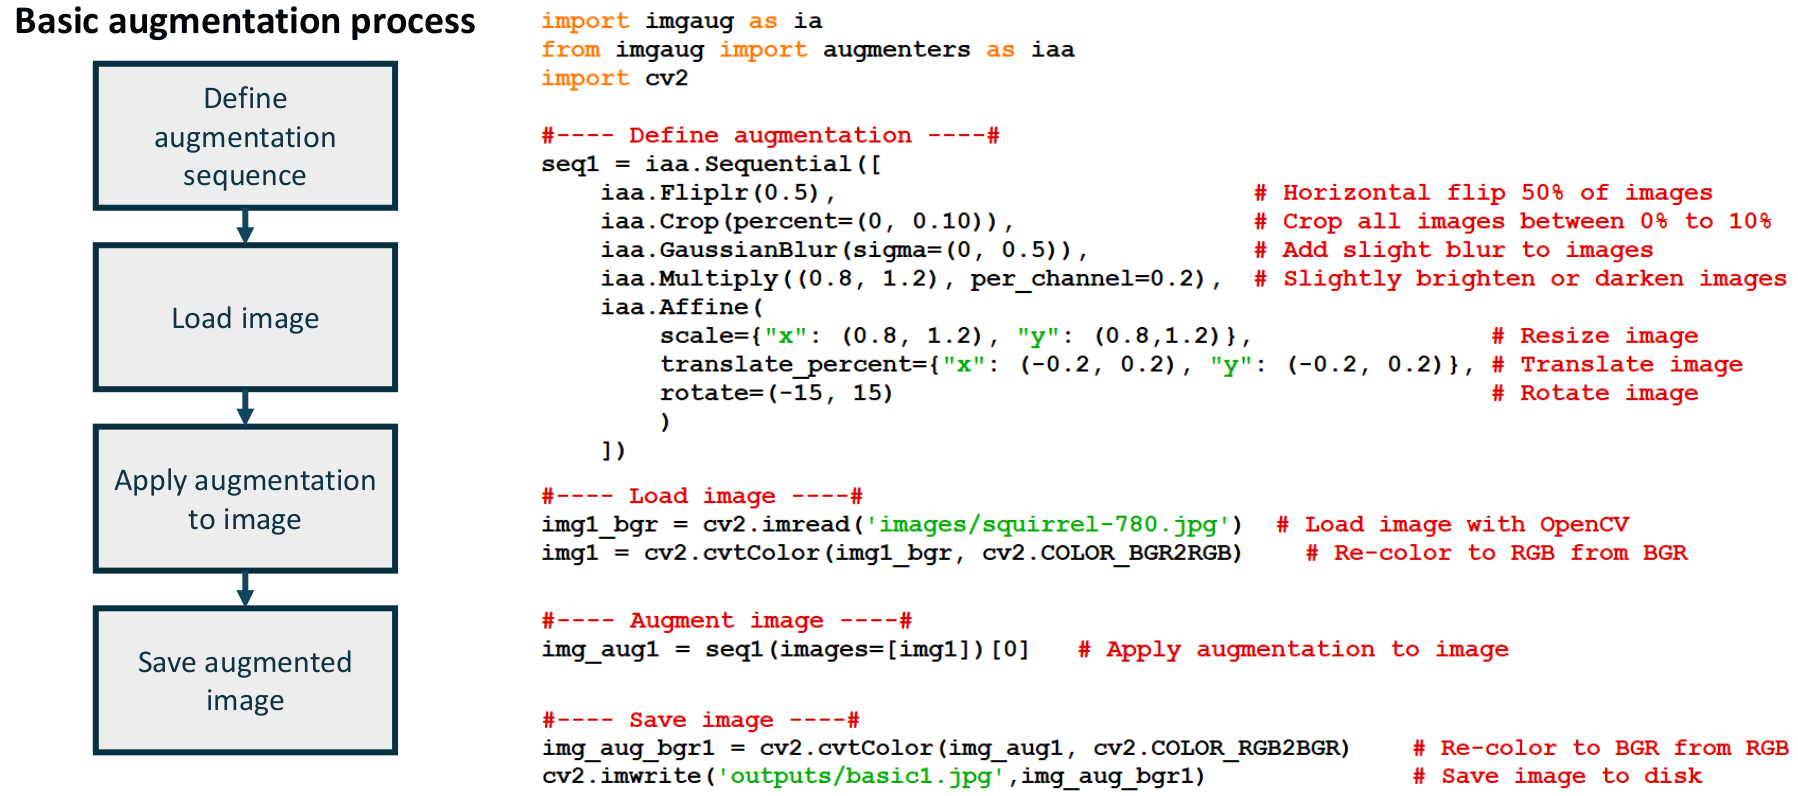
\includegraphics[width=14cm]{imgs/basic_augmentation_process.png}
\end{figure}
\end{frame}


%%%%%%%%%%%%%%%%%%%%%%%%%%%%%%%%%%%%%%%%%%%%%%%%%%%%%%%%%%%%%%%%%%%%%%%%%%%%%%%%%%%%%%%%%%%%%%%%%%%%%%%%%%%%%%%%

\begin{frame}{Object Detection Data Augmentation}{Example}
\begin{figure}[h]
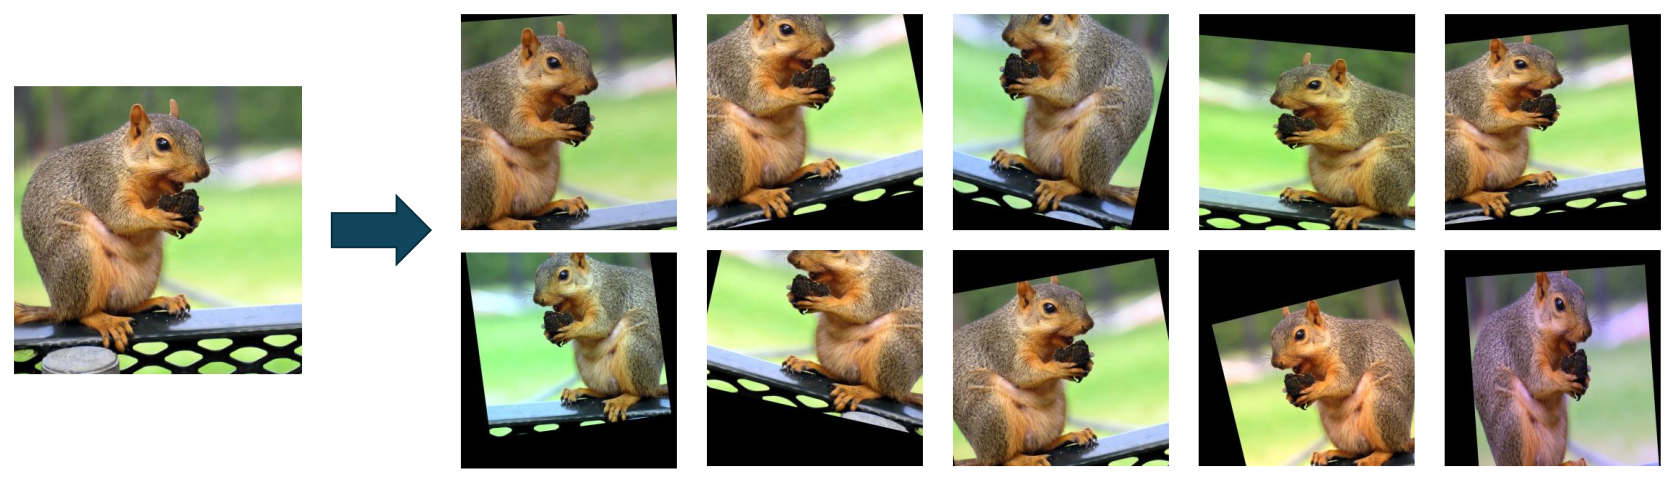
\includegraphics[width=14cm]{imgs/example.png}
\end{figure}
\end{frame}

%%%%%%%%%%%%%%%%%%%%%%%%%%%%%%%%%%%%%%%%%%%%%%%%%%%%%%%%%%%%%%%%%%%%%%%%%%%%%%%%%%%%%%%%%%%%%%%%%%%%%%%%%%%%%%%%

\begin{frame}{Object Detection Data Augmentation}{Example}
\begin{figure}[h]
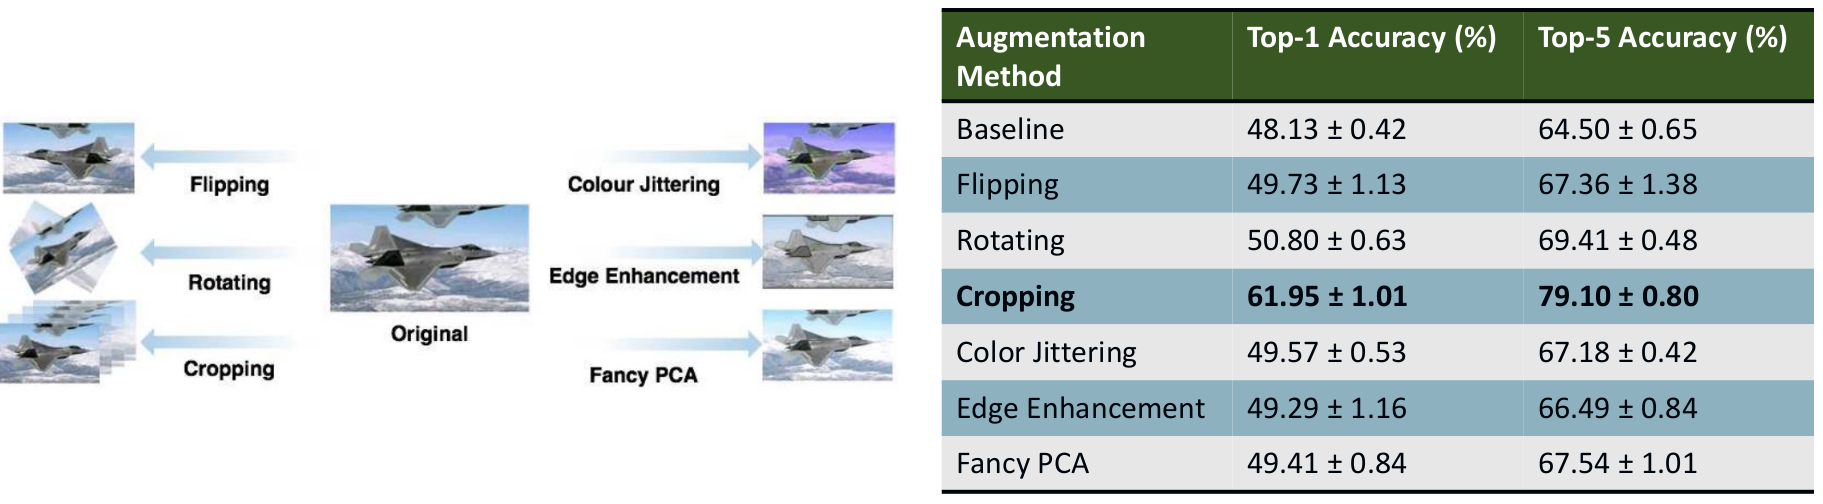
\includegraphics[width=14cm]{imgs/example2.png}
\end{figure}
\end{frame}

%%%%%%%%%%%%%%%%%%%%%%%%%%%%%%%%%%%%%%%%%%%%%%%%%%%%%%%%%%%%%%%%%%%%%%%%%%%%%%%%%%%%%%%%%%%%%%%%%%%%%%%%%%%%%%%%
\section{Experimento}
%%%%%%%%%%%%%%%%%%%%%%%%%%%%%%%%%%%%%%%%%%%%%%%%%%%%%%%%%%%%%%%%%%%%%%%%%%%%%%%%%%%%%%%%%%%%%%%%%%%%%%%%%%%%%%%%

\begin{frame}{Object Detection Data Augmentation}{Experimento}
Experiment to demonstrate how augmentation can improve performance
\begin{itemize}
\item 3-class model: Bird, squirrel, and raccoon (stuffed animals)
\item Start with unbalanced dataset: 5 bird images, 30 squirrel images, 30 raccoon images
\item Use augmentation to create 25 more bird images
\item Train models using unbalanced and augmented dataset, compare performance
\end{itemize}
\end{frame}

%%%%%%%%%%%%%%%%%%%%%%%%%%%%%%%%%%%%%%%%%%%%%%%%%%%%%%%%%%%%%%%%%%%%%%%%%%%%%%%%%%%%%%%%%%%%%%%%%%%%%%%%%%%%%%%%

\begin{frame}{Object Detection Data Augmentation}{Experimento}

\begin{figure}[h]
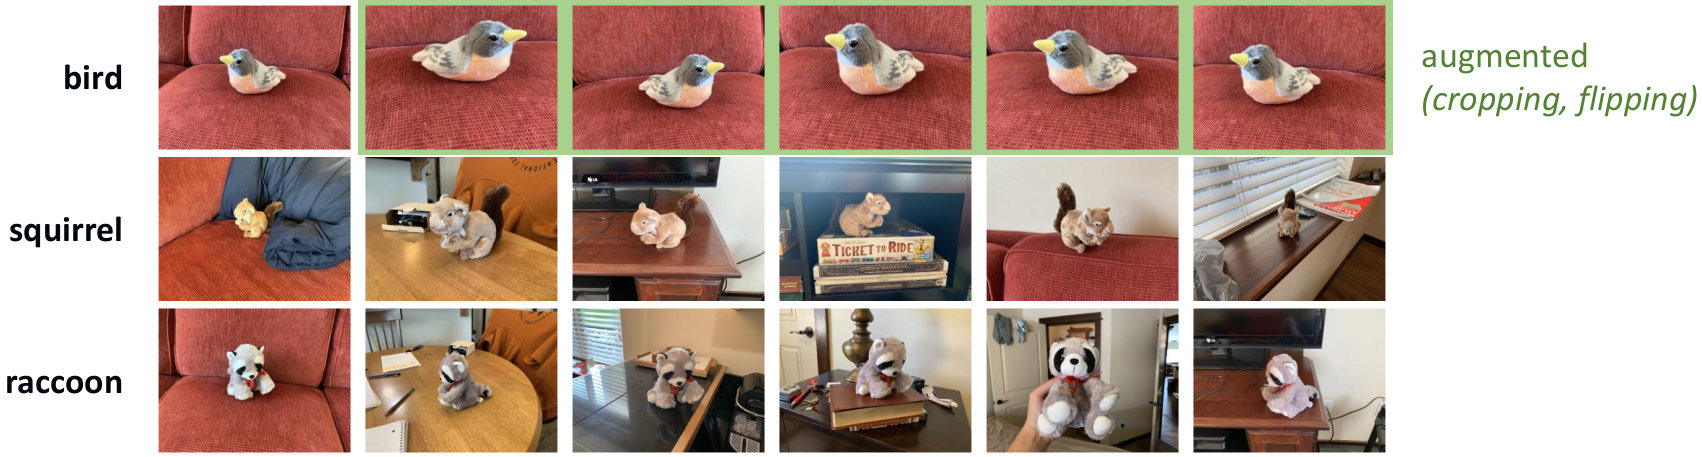
\includegraphics[width=14cm]{imgs/experiment.png}
\end{figure}
\end{frame}

%%%%%%%%%%%%%%%%%%%%%%%%%%%%%%%%%%%%%%%%%%%%%%%%%%%%%%%%%%%%%%%%%%%%%%%%%%%%%%%%%%%%%%%%%%%%%%%%%%%%%%%%%%%%%%%%

\begin{frame}{Object Detection Data Augmentation}{Experimento}

\begin{figure}[h]
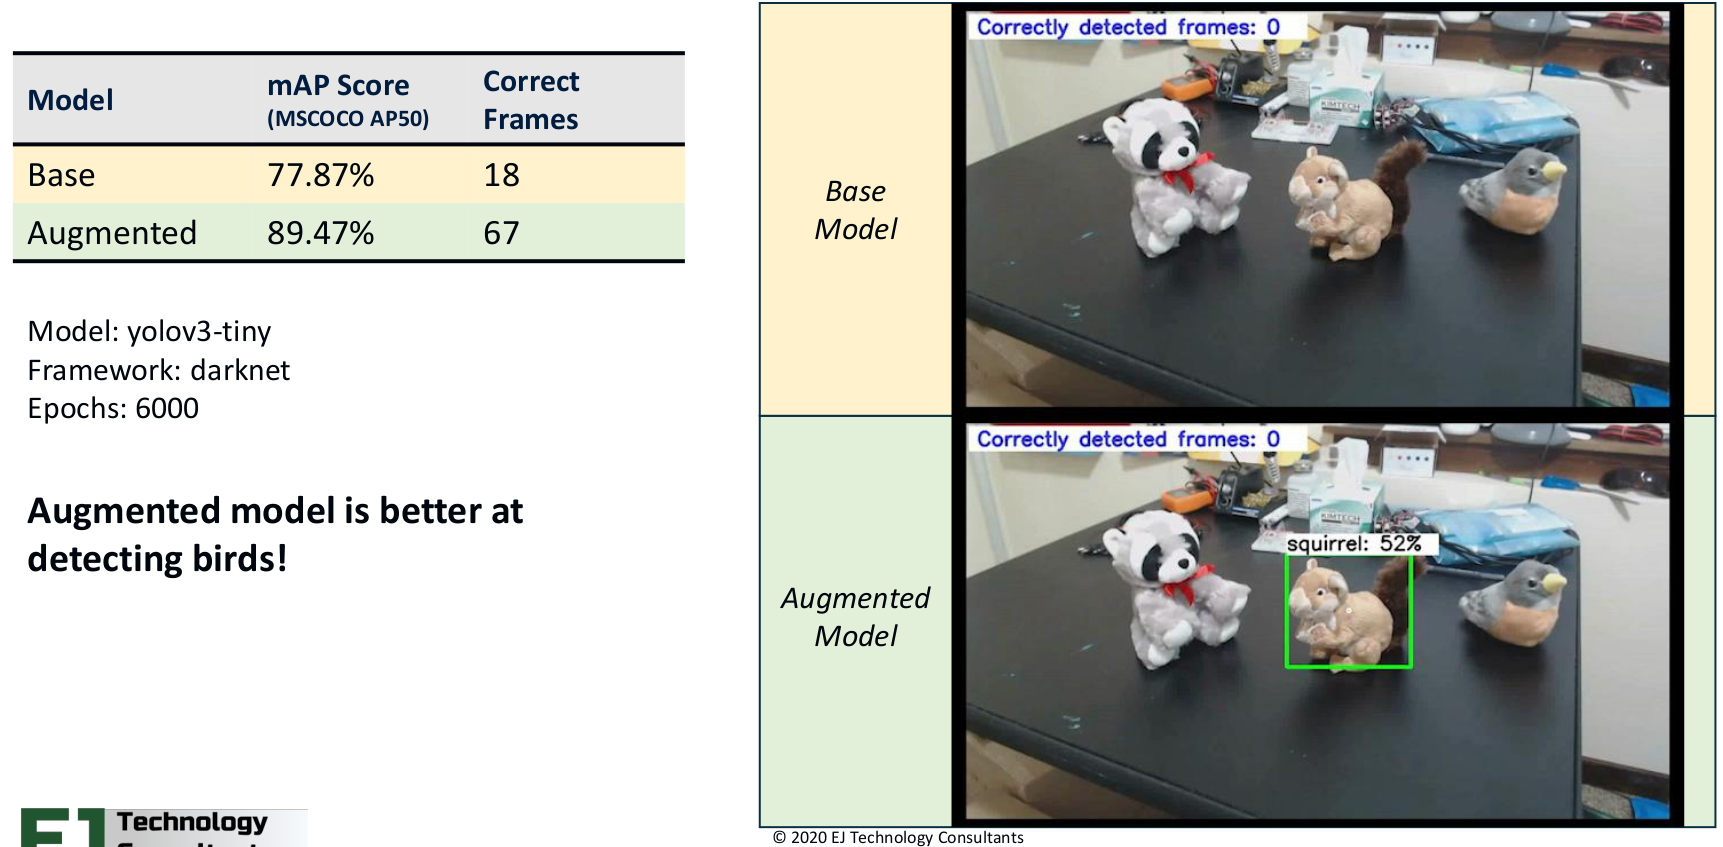
\includegraphics[width=14cm]{imgs/experiment_results.png}
\end{figure}
\end{frame}

%%%%%%%%%%%%%%%%%%%%%%%%%%%%%%%%%%%%%%%%%%%%%%%%%%%%%%%%%%%%%%%%%%%%%%%%%%%%%%%%%%%%%%%%%%%%%%%%%%%%%%%%%%%%%%%%
\section{Considerac�es}
%%%%%%%%%%%%%%%%%%%%%%%%%%%%%%%%%%%%%%%%%%%%%%%%%%%%%%%%%%%%%%%%%%%%%%%%%%%%%%%%%%%%%%%%%%%%%%%%%%%%%%%%%%%%%%%%

\begin{frame}{Considerac�es}
\begin{itemize}
\item When to Perform Augmentation?
\begin{itemize}
\item Augment images before training
\begin{itemize}
\item Reduces training pipeline overhead (speeds up training)
\item Can take considerable storage space
\end{itemize}
\end{itemize}
\begin{itemize}
\item Augment images during training
\begin{itemize}
\item Requires more processing power (slows down training)
\item Reduces and simplifies storage requirements
\item Increases statistical variation, better improvement in generalization
\end{itemize}
\end{itemize}
\item Which Dataset to Augment?
\begin{itemize}
\item Train: Yes ? allows network to learn robust features
\item Validation: No ? Unless planning to tweak hyperparameters during training
\item Test: No ? Test images should be from real-world conditions  
\end{itemize}
\end{itemize}
\end{frame}

%%%%%%%%%%%%%%%%%%%%%%%%%%%%%%%%%%%%%%%%%%%%%%%%%%%%%%%%%%%%%%%%%%%%%%%%%%%%%%%%%%%%%%%%%%%%%%%%%%%%%%%%%%%%%%%%

\begin{frame}{Considerac�es}
\begin{itemize}
\item Overall number of images
\begin{itemize}
\item Generally, more is better, but there?s an upper limit to effective dataset sizes
\item Dependent on application ? if used in wide variety of visual conditions, more images are needed
\item Pete Warden rule of thumb: 1000 images per class if training from scratch
\end{itemize}
\item Ratio of augmented to original images
\begin{itemize}
\item If only 50 images are used to create 5000 augmented images, model will be heavily biased towards 50 original
images
\item Ratio between 5:1 and 10:1 works well
\end{itemize}
\item Resolution of images
\begin{itemize}
\item Resolution should be similar to resolution of camera/video/images that will be used in application
\item Higher resolution requires much more memory during training
\end{itemize}
\end{itemize}
\end{frame}

%%%%%%%%%%%%%%%%%%%%%%%%%%%%%%%%%%%%%%%%%%%%%%%%%%%%%%%%%%%%%%%%%%%%%%%%%%%%%%%%%%%%%%%%%%%%%%%%%%%%%%%%%%%%%%%%

\begin{frame}{Object Detection Data Augmentation}{Limitac�es}
\begin{figure}[h]
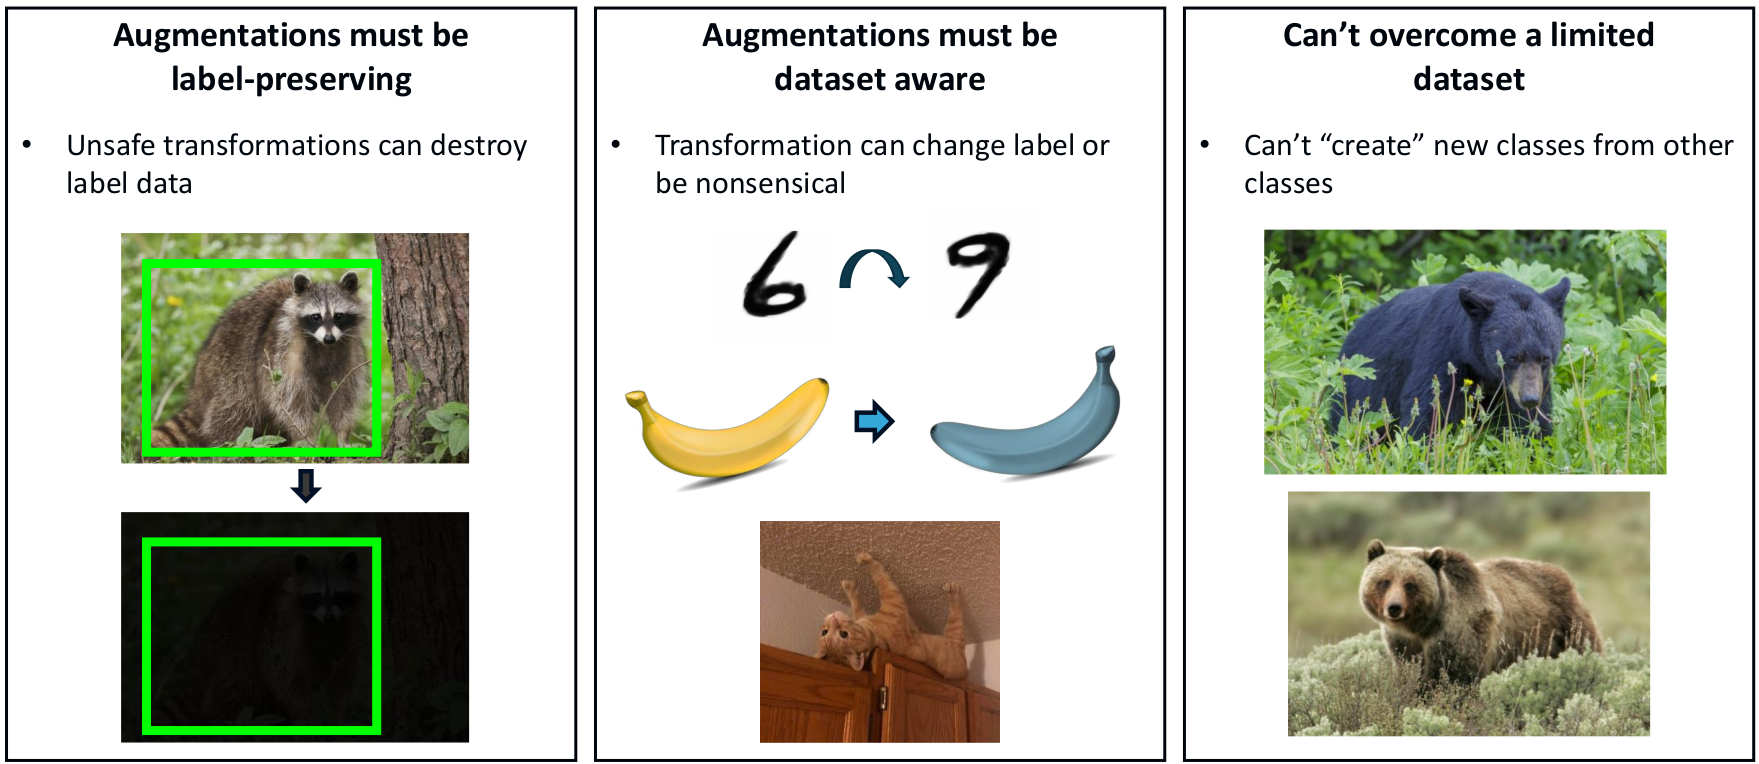
\includegraphics[width=14cm]{imgs/data_aug_limitations.png}
\end{figure}
\end{frame}

%%%%%%%%%%%%%%%%%%%%%%%%%%%%%%%%%%%%%%%%%%%%%%%%%%%%%%%%%%%%%%%%%%%%%%%%%%%%%%%%%%%%%%%%%%%%%%%%%%%%%%%%%%%%%%%%

\begin{frame}{Conclus�es}
\begin{itemize}
\item Data augmentation can increase model accuracy with minimal effort
\item Random background augmentation technique is very effective for static 2D objects
\item Need to consider when and where to apply augmentation, and how much
\item Data augmentation has some limitations
\end{itemize}
\end{frame}

%%%%%%%%%%%%%%%%%%%%%%%%%%%%%%%%%%%%%%%%%%%%%%%%%%%%%%%%%%%%%%%%%%%%%%%%%%%%%%%%%%%%%%%%%%%%%%%%%%%%%%%%%%%%%%%%

\begin{frame}{Referencias}
\begin{itemize}
\item Practical Image Data Augmentation Methods for Training Deep Learning Object Detection Models, a Presentation from EJ Technology Consultants 
  \begin{itemize}
  \item \url{https://www.edge-ai-vision.com/2021/01/practical-image-data-augmentation-methods-for-training-deep-learning-object-detection-models-a-presentation-from-ej-technology-consultants/}
  \end{itemize}   
\end{itemize}
\end{frame}

%%%%%%%%%%%%%%%%%%%%%%%%%%%%%%%%%%%%%%%%%%%%%%%%%%%%%%%%%%%%%%%%%%%%%%%%%%%%%%%%%%%%%%%%%%%%%%%%%%%%%%%%%%%%%%%%

\begin{frame}[plain]
  \titlepage
\end{frame}


\end{document}
